\documentclass{article}
\usepackage{graphicx}
\usepackage[rightcaption]{sidecap}
\graphicspath{ {./billeder/} }
\usepackage{amsmath,amsfonts,stmaryrd,amssymb}
\usepackage[ruled]{algorithm2e}
\usepackage[framemethod=tikz]{mdframed}
\usepackage{parskip}
\usepackage{nameref}
\usepackage{booktabs}
\usepackage{tabularx}
\usepackage{geometry}
\geometry{
	paper=a4paper,
	top=2.5cm,
	bottom=3cm,
	left=2.5cm,
	right=2.5cm,
	headheight=14pt,
	footskip=1.5cm,
	headsep=1.2cm,
	%showframe, % Uncomment to show how the type block is set on the page
}

\usepackage[utf8]{inputenc}
\usepackage[T1]{fontenc}
\usepackage{XCharter}
\usepackage{graphicx}

\author {Jesper Toplund}
\title{Roadmap for komponenter}
\date{}

\begin{document}
\maketitle

\vspace{20 mm}
\begin{quote}
    \textit{}
\end{quote}

\section{Baggrund}
Dette rapport er skrevet for nedfælge mine tanker og ideer angående arkitekturen i Web og Apps. Det skrevne er baseret på det indblik jeg har fået i arkitekturen over de sidste par måneder. Der vil helt klart være nuancer i den eksisterende arkitektur som der ikke er taget højde for og dermed er der formentligt konklusioner der er baseret på mangelfuld information. Dette dokument skal helt bestemt ses som et levende dokument, som over tid skal holdes opdateret.

\subsection{Formål}
Det primære formål med rapporten er at ridse et roadmap op for hvad vi bør fokusere på hvis vi gerne vil opnå en sammenhængende, tidssvarende og vedligeholdbar arkitektur.

\subsection{Omfang}
Denne rapport er skrevet ud fra informationerne i DR systemkatalog og de betragtninger der er blevet gjort i forbindelse med arkitektur rapporten fra Eksponent. Estimater og overslag der er angivet i rapporten er foretaget ud fra et kvalificeret bud på besvær og omkostninger og ikke ud fra en detaljeret analyse af hvert enkelt projekt. Mere præcise estimater vil være mulige for hvert delopgave, men er uden for scope af denne rapport.
% highlevel gennemgang. mere præcise estimater kræver mere konkret gennemgang af de enkelte elementer i den samlede arkitektur

\section{Executive summary}
Arkitekturen i Web og Apps bærer præg af at have vokset organisk frem. Når et forretningsproblem har vist sig, er der blevet lavet en løsning på problemet ud fra de for hånden værende ressourcer og kompetencer, uden hensyntagen til hvordan løsningen passer ind i resten af systemlandskabet. Det har resulteret i at vi i dag har mange eksempler på parallelle implementeringer, på systemer der ikke kan vedligeholdes, på ukendt aftagerlandskab og på fragmenteret infrastruktur.

De vigtigste skridt vi skal igennem er følgende:
\begin{itemize}
\item Design af gennemgående datamodel
\item Konsolidering af infrastruktur
\item Omskrivning af forældede produkter
\item Sikre DevOps fundament
\end{itemize}
Vi skulle gerne ende op med en arkitektur, hvor det er muligt at have styr på vores aftagerlandskab. Vi skal også have mulighed for hurtig kommunikation imellem interne komponenter via sikret og afgrænset netværk. Det skal være muligt at teste komponenter individuelt og i et sammenhængende produktionslignende test setup.
%TODO grov estimat?

\section{Generelt forarbejde}
\subsection{Indholds datamodel}
Noget af det vigtigste for at få arkitekturen til at hænge sammen er at vi får etableret en generel og gennemgående datamodel, som kan være med til at sikre at alle vores komponenter kan kommunikere på tværs. Det er et vigtigt stykke forarbejde som både bidrager til muligheden for at rydde op i den hårknude som arkitekturen er nu og gør det muligt at sikre at nyudviklede komponenter kan benyttes på tværs. Det kommer til at kræve en del arbejde at få etableret denne datamodel og derefter at få de forskellige systemer tilpasset til denne datamodel.

Det anbefales at vi starter med at udarbejde en så dækkende model som muligt, gerne en der læner sig op ad den som allerede benyttes af Steffi. Dermed får vi et centralt udgangspunkt som, når det bredes ud, kan bruges som samlingspunkt om vores content aggregation service.

Datamodellen skal ikke nødvendigvis implementeres på tværs af hele dr.dk fra starten af, men det vil være til stor gavn hvis vi kan arbejde os i retning af en fælles datamodel i alle fremtidige større ændringer af systemerne.
Udarbejdelse af Datamodellen bør ske inden næste store ændring i et af de centrale indholdsbærende datalag (mimer, steffi, Hydra, nyhedsapp eller lignende).

Udarbejdelse af datamodellen vil tage ca 2 mandeuger.


\subsection{URN / URL}
Hvis vi samtidigt med opdateringen af datamodellen også kikker på DR URN, så kan vi sikre at det er muligt at unikt identificere indhold på tværs af systemer uden kendskab til systemlandskabet. 
%TODO Der mangler helt sikkert info her 


\subsection{Underliggende infrastruktur}
Alt indhold på dr.dk serves i dag igennem Akamai CDN. Akamai fungerer som content delivery network, ddos beskyttelse og cache lag. I tilfælde af udfald hos DR.dk er cache hos Akamai sat til at blive ved med at serve gammel data ind til vi igen er i stand til at besvare på forespørgsler hos DR.dk. Det betyder at forlængede svartider eller korte nedbrud ikke nødvendigvis bliver bemærket hos slutbrugeren.

Infrastrukturen som i dag driver dr.dk har et par fordele men også en række ulemper. Hvert team har valgt hosting og teknologi ud fra hvad de kender til og deres ønsker om funktionalitet. Det betyder at vi i dag har dele af dr.dk hostet på 4 forskellige cloud platforme.
For at en artikel kan udkomme på dr.dk forsiden og i nyhedsapp skal der udveksles data på tværs af alle 4 skyer.

Kommunikations udfald eller nedbrud hos en af cloud udbyderne vil i de fleste tilfælde betyde at vi ikke kan udkomme med nye artikler. Der er ingen driftsmæssig fordel ved at vi har baseret vores infrastruktur på 4 forskellige skyer, da udgivelse af en artikel vil fejle lige meget hvilket led i kæden der knækker. 
%TODO  
% Kort blabla om de mange skyer, distribueret model og sårbarheder.  Man skulle tro nuværende setup giver stor stabilitet men reelt er antallet af fejlkilder blot forøget, mens fejlhåndteringen er skiftet fra "worst subsystem"?? til "last succesfull response"??

\subsection{parallelliseret og distribueret system}
Vi har en forpligtigelse om at kunne udkomme med nyheder og varslinger hele tiden og med kort varsel. Det stiller selvfølgeligt krav til vores systemers oppetid. Jo tættere koblet et system er, jo mere sårbar er det over for nedbrud et eller andet sted i afhængighedskæden.
De systemer vi selv hoster og drifter bør sikres i det omfang det er muligt. Jeg vil foreslå at vi kikker grundigt på et parallelt sky setup, så vi f.eks. har en primær region (europe-west2) hvor der er veldefinerede skalerings regler og overvågning sat op. Vi kan samtidigt have en sekundær sky sat op i en anden region (f.eks. europe-west4) som er skaleret helt i bund og ingen trafik varetager.
Ved nedbrud i den primære region kan vi skifte til den sekundære og lade den skalere op.

%TODO. Bemærkning om parallel monteret sky. Hvis vi har alt kørende i en region, så kan vi risikere at alt går ned hvis den region får kritiske nok fejl. Vi bør have en aktiv instans kørende på en anden region, som er skaleret helt i bund men er klar til at skalere. Ved kritiske fejl i en region kan vi så skifte over på en anden region. 


\subsection{DevOps kulturen styrkes}
Teams i Web og Apps lever på mange punkter op til DevOps tankegangen. De enkelte teams er i stand til at drifte, udvikle, teste og deploye deres produkter.  Der er dog en række punkter som helt klart kan forbedres.

\subsubsection{Ensretning af pipeline}
Med henblik på at lette deployment til både test miljøer og produktions miljøer vil det være en stor fordel hvis deployment kunne foregå fra et fælles værktøj. 
Ideelt set skal det være muligt at deploye et komplet miljø til enten test eller produktion fra et centralt sted. Det må meget gerne være muligt at have et aktivt produktionssystem, et inaktivt produktionssystem, et aktivt test system og mulighed for at deploye dedikerede testsystemer. 

\subsubsection{Fælles overvågning}
Udviklerne i de enkelte teams er specialister i deres egne systemer og er som sådan de bedst egnede til at fejl finde og vedligeholde deres systemer. Det er dog ikke det samme som at udviklerne er de bedst egnede til at overvåge og fejl finde i infrastrukturen som systemerne kører på. Ideelt skal vores systemer køre på en fælles platform, som der kan overvåges centralt.
Ideelt set burde platformen overvåges centralt, med veldefinerede alarmer på alle miljøer. I tilfælde af nedbrud på et miljø bør overvågningen have en drejebog på hvilke skridt der kan foretages for at afhjælpe problemerne.
For at opnå det er der behov for følgende:
\begin{itemize}
\item konsolidering af driftsmiljøer
\item velbeskrevne overvågnings parametre
\item velbeskrevet drejebog for afhjælpning af problemer
\item velbeskrevet eskalerings muligheder af problemer
\end{itemize}

Udviklerne i de enkelte teams har ansvaret for udvikling tests og vedligeholdelse af deres systemer. Udviklerne skal ligeledes sørge for at der opsættes overvågningspunkter, så der kan rapporteres systemstatus til overvågningen samt drejebøger for hvordan almindelige fejl kan afhjælpes.
DevOps afdelingen skal stå for udvikling af de nødvendige værktøjer og skal have det formelle ejerskab af infrastrukturen. Hvis der er nedbrud på netværk, Hosting eller andre infrastruktur komponenter, så skal dette løses af ejeren af infrastrukturen.
Overvågningen kan varetages af "Infra". Denne overvågning skal være af både infrastruktur og overvågningspunkter der leveres af udviklerne i de enkelte udviklingsteams. Da hverken DevOps eller de enkelte udviklingsteams har døgnovervågnings muligheder er Infra en af de eneste muligheder der er for at afhjælpe problemer på platformen uden for normal arbejdstid.



* DevOps tankegangen er et strålende bud på en løsning af 3 delingen mellem infrastruktur, drift og udvikling.
* Devops skal styrkes i de enkelte udviklings teams.
	De skal kunne lave hyppige releases.
	De skal kunne lave sikre releases.
	De skal kunne overvåge deres applikationer.
	De skal kunne fejlfinde i deres applikationer på tværs af hele platformen.
Centraliseret overvågning af infrastrukturen.
	De enkelte teams i Web og apps skal ikke være ansvarlige for overvågning af hele infrastrukturen.
%TODO. Dette er nok det vigtigste afsnit. Her skal skrives MEGET


\section{Analyse af komponenter}

\subsection{Akamai}
\begin{figure}[h]
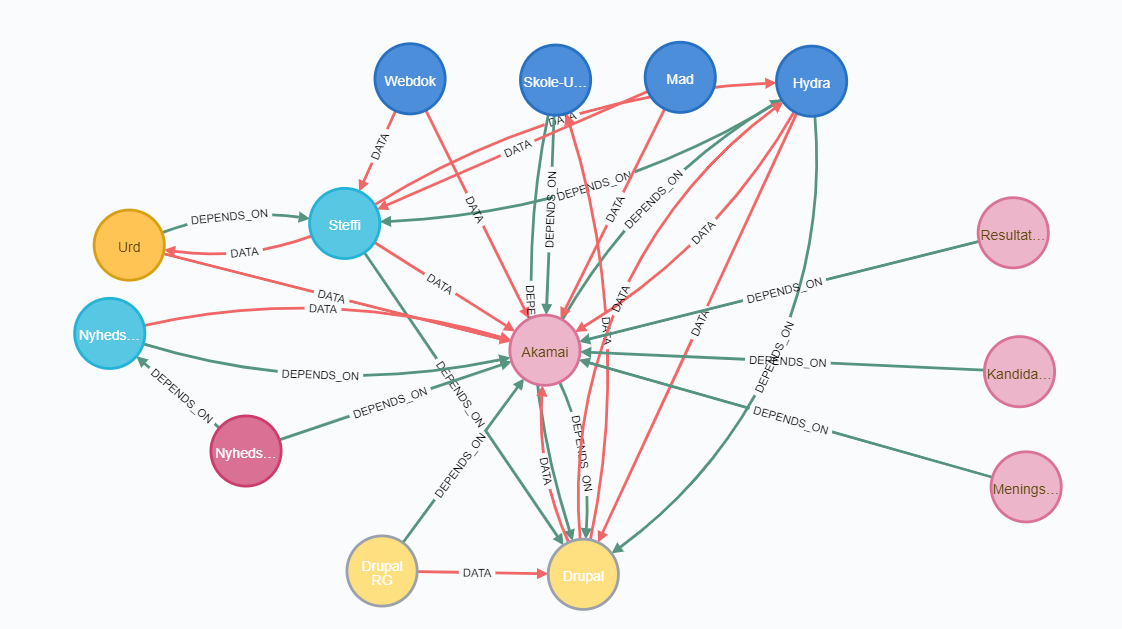
\includegraphics[width=300pt]{Akamai.PNG}
\caption{MATCH (x\{name:'Akamai'\})- -(y) RETURN x,y}
\end{figure}
\subsubsection{Kort beskrivelse}
Akamai benyttes som det primære CDN (content delivery Network). 
Det er dermed ikke et produkt som er udviklet hverken af eller for DR, 
men et produkt som vi er afhængige af. 
\subsubsection{Anbefalet handling}
Akamai som CDN udfylder fint de behov som DR har. 

Vi kan med fordel kikke på om vi benytter fornuftige cache timeouts eller om vores hjemmeside er struktureret til at få mest muligt ud af CDN.
\subsubsection{Overslag}
Indgår ikke som sådan i roadmap.


\subsection{Hydra}
\begin{figure}[h]
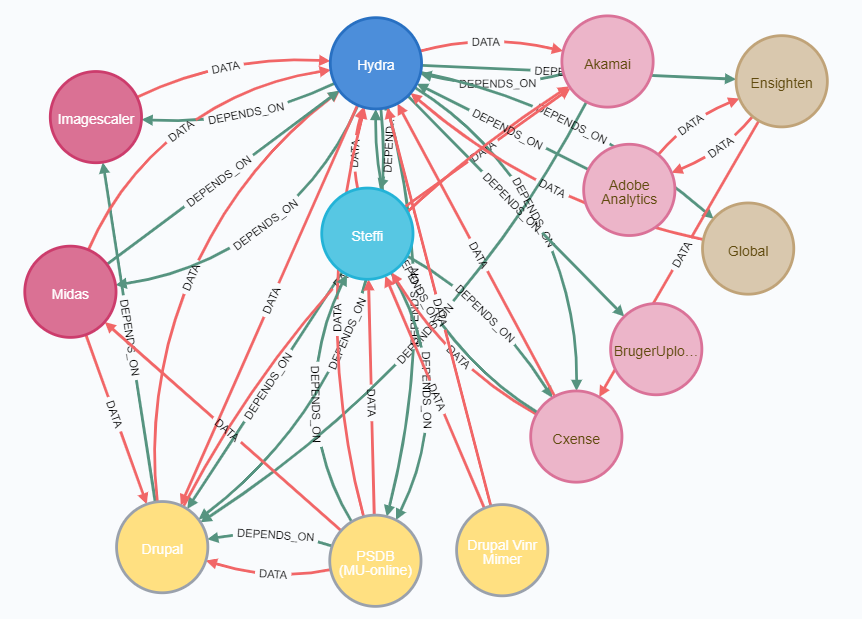
\includegraphics[width=300pt]{Hydra.PNG}
\caption{MATCH (x\{name:'Hydra'\})- -(y) RETURN x,y}
\end{figure}
\subsubsection{Kort beskrivelse}
Web-frontend, der varetager indholdsvisning for artikler og forsider. Anvender Drupal-visning til sider, der endnu ikke understøttes af Hydra.
Ovenstående figur viser at der er et højt antal afhængigheder til mange systemer. Det skal undersøges nærmere om de alle er aktuelle.
\subsubsection{Anbefalet handling}
Hydra er beskrevet som at den direkte henter data fra og sender data til Drupal. Er det korrekt, så springer den flere lag over i referencearkitekturen.
Hydra burde kun afhænge af platform utilities, platform services, product services eller content aggregation.
% TODO Verificer at alle de beskrevne afhængigheder også er aktuelle afhængigheder.
\subsubsection{Overslag}
Afklaring nødvendigt før det kan estimeres.


\subsection{Steffi}
\begin{figure}[h]
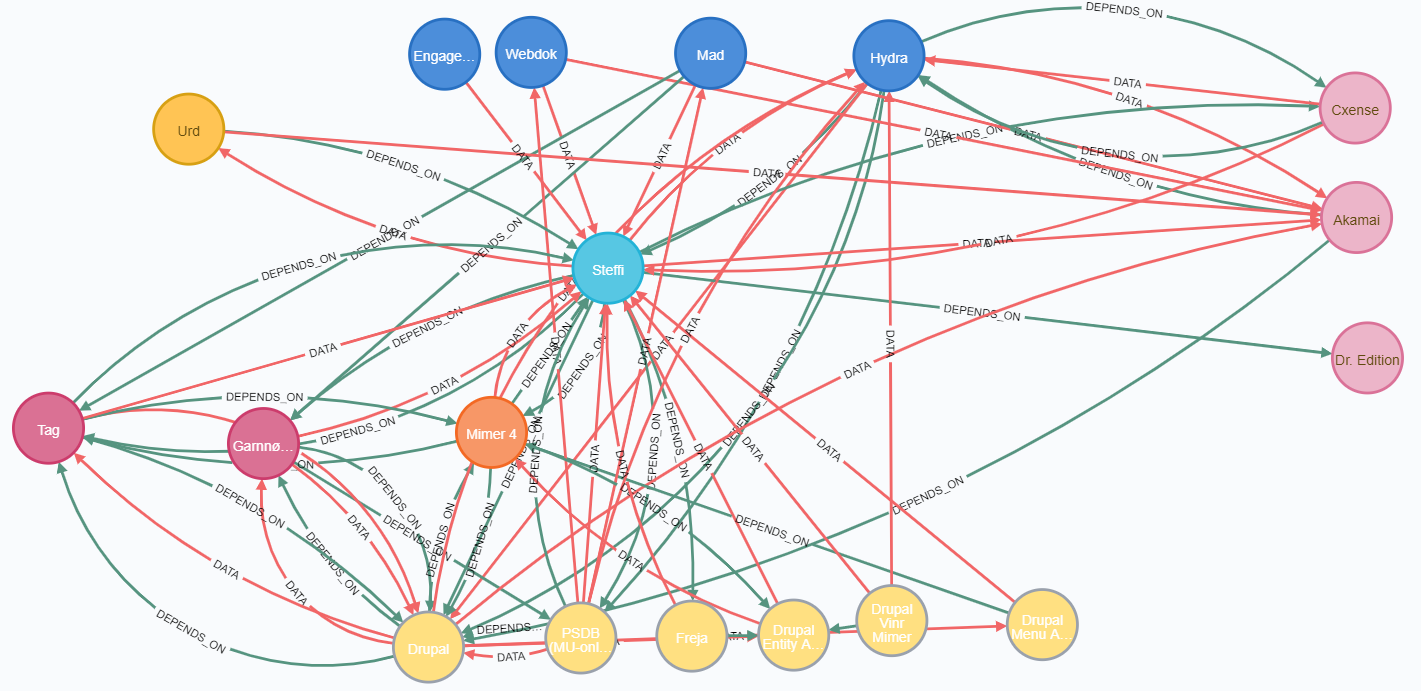
\includegraphics[width=300pt]{Steffi.PNG}
\caption{MATCH (x\{name:'Steffi'\})- -(y) RETURN x,y}
\end{figure}
\subsubsection{Kort beskrivelse}
Forespørgselslag, der tilbyder GraphQL-grænseflader til frontendapplikationer.
benyttes Content aggregering.
\subsubsection{Anbefalet handling}
\subsubsection{Overslag}


\subsection{Talentholdet}
\begin{figure}[h]
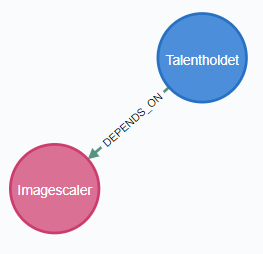
\includegraphics[width=300pt]{Talentholdet.PNG}
\caption{MATCH (x\{name:'Talentholdet'\})- -(y) RETURN x,y}
\end{figure}
\subsubsection{Kort beskrivelse}
Talentholdet er en rekrutteringsplatform for nye talenter til DR. Talentholdet har sin egen database hvori den gemmer personidentificerbar data i krypteret form. Talentholdet afhænger af Imagescaler
\subsubsection{Anbefalet handling}
Talentholdet udfører en mindre opgave som det er muligt at diskutere værdien af. Vi bør få afklaret med forretningen om vi eventuelt kan pensionere programmet. Der er en del kodegæld i programmet og GDPR sletninger er en manuel process.
Prioriteten af Talentholdet er dog ret lav, så den manuelle process kan tolereres.
\subsubsection{Overslag}
N/A

\subsection{Elements}
\begin{figure}[h]
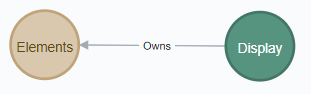
\includegraphics[width=200pt]{Elements.PNG}
\caption{MATCH (x\{name:'Elements'\})- -(y) RETURN x,y}
\end{figure}
\subsubsection{Kort beskrivelse}
Elements er DR's centrale komponentbibliotek, som består af FE komponenter. Elements er kodet i React. Elements benyttes af en række af vores Frontend products.
\subsubsection{Anbefalet handling}
Elements benyttes en række af vores Frontend products og passer fint ind i vores reference arkitektur
\subsubsection{Overslag}
N/A

\subsection{Webdok}
\begin{figure}[h]
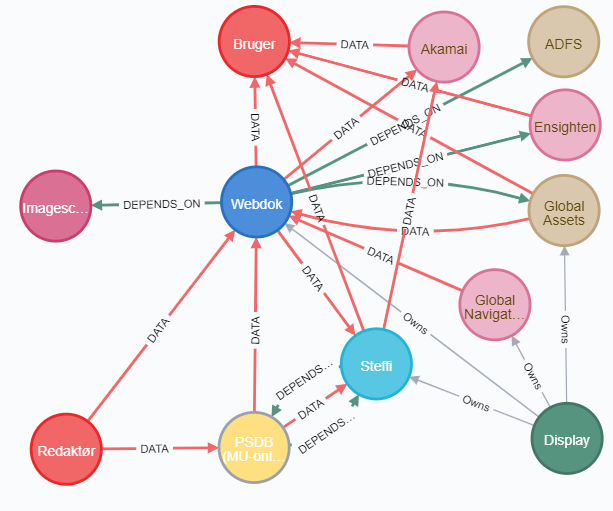
\includegraphics[width=300pt]{Webdok.PNG}
\caption{MATCH (x\{name:'Webdok'\})- -(y) RETURN x,y}
\end{figure}
\subsubsection{Kort beskrivelse}
CMS og præsentation af featureartikler i særformater.	
Præsentationslag (Node.js) trækker data fra API (.NET). Redaktørgrænseflade er bygget ind i præsentationslaget.
\subsubsection{Anbefalet handling}
Hvordan Webdok er flettet ind i vores nuværende arkitektur skal undersøges nærmere. Dokumentationen som den står nu giver et lidt mudret billede
% TODO
\subsubsection{Overslag}
Ukendt.


\subsection{Skole-Undervisning}
\begin{figure}[h]
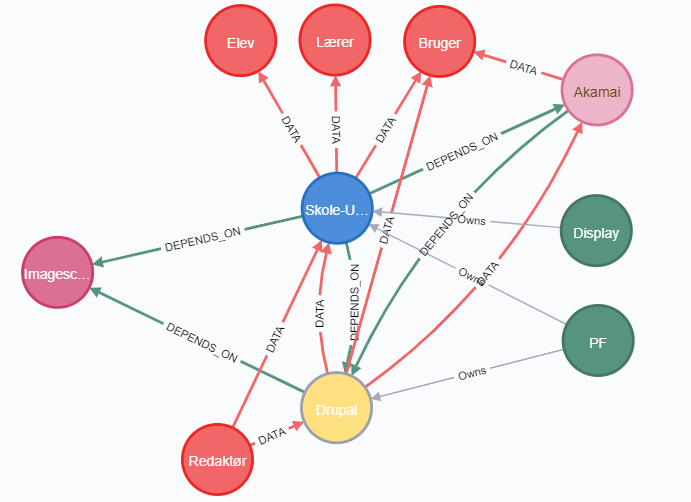
\includegraphics[width=300pt]{Skole-Undervisning.PNG}
\caption{MATCH (x\{name:'Skole-Undervisning'\})- -(y) RETURN x,y}
\end{figure}
\subsubsection{Kort beskrivelse}
Skole og Undervisning er et site, der formidler undervisningsforløb og undervisningsmateriale til Skoler.  Sitet er opbygget i Drupal, men har en række specialløsninger konstrueret for at kunne samle temaer og autogenerere faktabokse etc. 
\subsubsection{Anbefalet handling}
Skole-Undervisning passer ikke ind i referencearkitekturen, idet den udgør sin helt egen silo og udstiller data direkte til slutbrugere via Akamai. 
Afhængigt af levetiden for projektet (gartner Time model) skal vi overveje hvad vi gør ved projektet.
\subsubsection{Overslag}
Afklaring mangler.
%TODO

\subsection{Mad}
\begin{figure}[h]
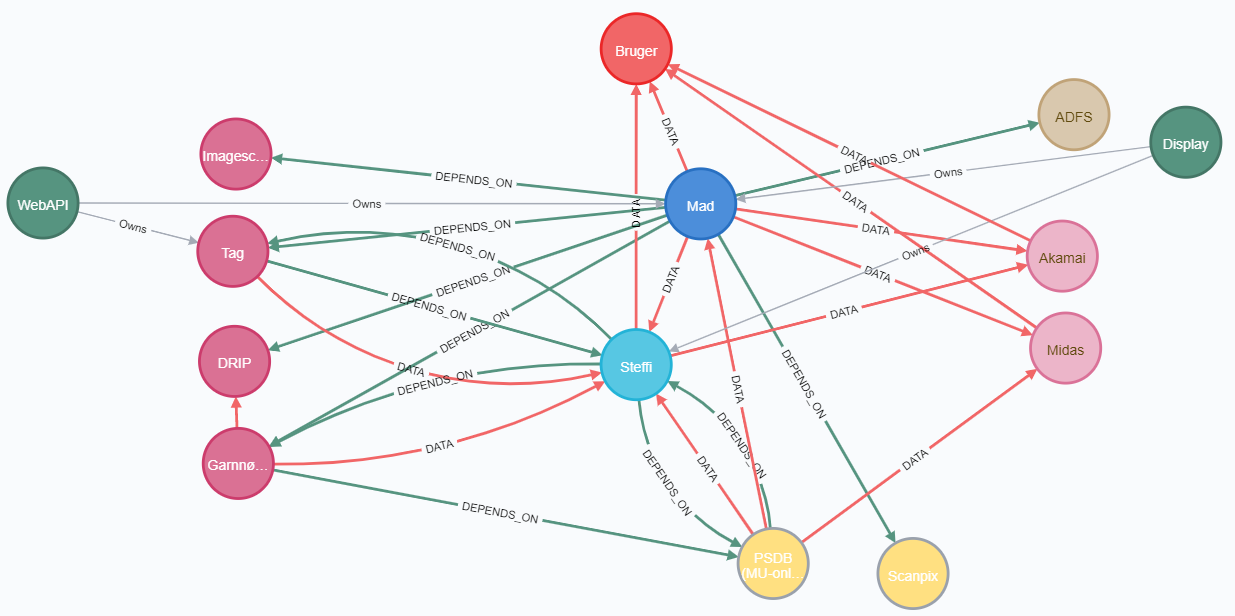
\includegraphics[width=300pt]{Mad.PNG}
\caption{MATCH (x\{name:'Mad'\})- -(y) RETURN x,y}
\end{figure}
\subsubsection{Kort beskrivelse}
Mad er en applikation, der håndterer opskrifter, artikler og opskriftssamlinger. Mad er bygget som Headless Drupal med egen RG til opskrifter. Artikler publiceres gennem Drupal. 
\subsubsection{Anbefalet handling}
Mad passer ikke helt ind i referencearkitekturen som beskrevet. Om det er en mangel i dokumentationen eller i arkitekturen skal undersøges. (hvorfor tilgår Steffi Mad direkte og ikke igennem f.eks. Mimer?)
\subsubsection{Overslag}
Afklaring mangler
%TODO

\subsection{Nyhedsapp-Frontend}
\begin{figure}[h]
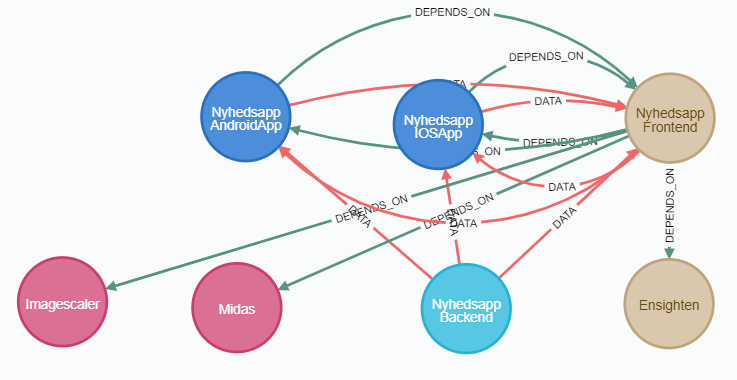
\includegraphics[width=300pt]{Nyhedsapp-Frontend.PNG}
\caption{MATCH (x\{name:'Nyhedsapp Frontend'\})- -(y) RETURN x,y}
\end{figure}
\subsubsection{Kort beskrivelse}
Præsentationslag for indhold i Nyhedsapp, således at visningen mellem iOS og Android er homogen, samt har lignende homogenitet til visningen på DR.dk
Nyhedsapp-Frontend er ikke en selvstændig applikation, men et delt kodelag der anvendes af IOS og Android udgaven af nyhedsappen. 
\subsubsection{Anbefalet handling}
Nyhedsapp-Frontend er en parallel implementering i forhold til Elements. Hvis der er ændringer i visningen af en artikel der kan vises både i nyhedsapp og på web, så skal der foretages ændringer i både Elements og Nyhedsapp-Frontend. Ved en renovation af Nyhedsapp-Frontend bør det undersøges om vi kan benytte en fælles kodebase til definition af visning.
\subsubsection{Overslag}
%TODO Sammensmeltning med Elements??
N/A

\subsection{Nyhedsapp IOS}
\begin{figure}[h]
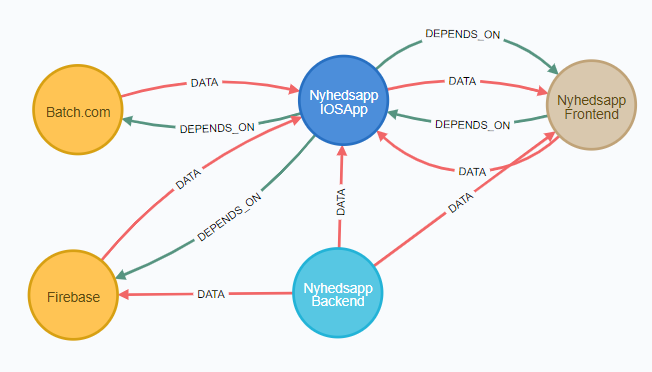
\includegraphics[width=300pt]{Nyhedsapp-IOS.PNG}
\caption{MATCH (x\{name:'Nyhedsapp IOSApp'\})- -(y) RETURN x,y}
\end{figure}
\subsubsection{Kort beskrivelse}
Afvikler Nyhedsapp Frontend, integrerer til iOS-native funktionalitet
\subsubsection{Anbefalet handling}
Nyhedsapp til både IOS og Android overholder referencearkitekturen. Der er måske ønsker om at opdatere applikationerne så de får et mere moderne udtryk på telefonerne. Dette ønske er dog et forretningsdrevet ønske og ikke en nødvendighed set ud fra reference arkitekturen
\subsubsection{Overslag}
Ingen ændringer nødvendige

\subsection{Nyhedsapp AndroidApp}
\begin{figure}[h]
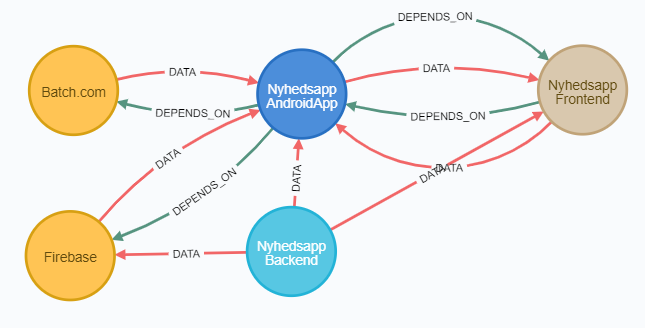
\includegraphics[width=300pt]{Nyhedsapp-Android.PNG}
\caption{MATCH (x\{name:'Nyhedsapp AndroidApp'\})- -(y) RETURN x,y}
\end{figure}
\subsubsection{Kort beskrivelse}
Native Android-wrapper, der afvikler Nyhedsapp Frontend
\subsubsection{Anbefalet handling}
Nyhedsapp til både IOS og Android overholder referencearkitekturen. Der er måske ønsker om at opdatere applikationerne så de får et mere moderne udtryk på telefonerne. Dette ønske er dog et forretningsdrevet ønske og ikke en nødvendighed set ud fra reference arkitekturen
\subsubsection{Overslag}
Ingen ændringer nødvendige


\subsection{Batch.com}
\begin{figure}[h]
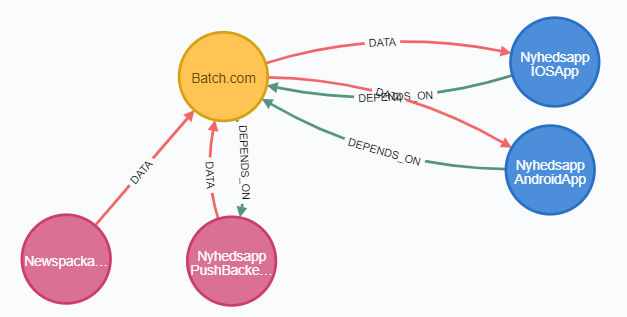
\includegraphics[width=300pt]{Batch-com.PNG}
\caption{MATCH (x\{name:'Batch.com'\})- -(y) RETURN x,y}
\end{figure}
\subsubsection{Kort beskrivelse}
SaaS tejneste der benyttes til push af beskeder til NyhedsApp
Distribuerer data til Nyhedsapp-instanser, med mulighed for dublikeringskontrol så den samme enhed kun modtager data én gang, og ligeledes en opfølgningsmulighed så devices der var utilgængelige på udsendelsestidspunktet, opdateres når de er tilgængelige igen
\subsubsection{Anbefalet handling}
Tjenesten passer ind i vores referencearkitektur. Om Batch.com bliver ved med at være den bedste løsning for push af beskeder vil vi ikke tage stilling til i dette dokument.
\subsubsection{Overslag}
Ingen ændringer nødvendige


\subsection{Firebase}
\begin{figure}[h]
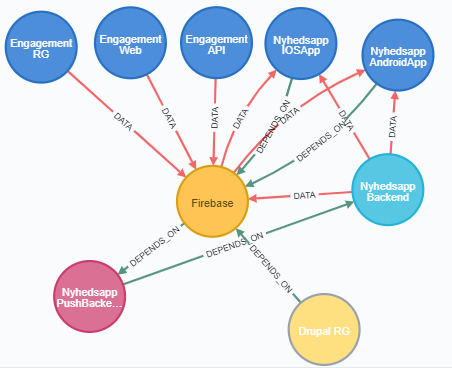
\includegraphics[width=300pt]{Firebase.PNG}
\caption{MATCH (x\{name:'Firebase'\})- -(y) RETURN x,y}
\end{figure}
\subsubsection{Kort beskrivelse}
SaaS tjeneste der benyttes til Pusg service af flere applikationer:
Nyhedsapp, Drupal RG ("hvem er inde på min artikel")
\subsubsection{Anbefalet handling}
Tjenesten passer ind i vores referencearkitektur. Om Firebase bliver ved med at være den bedste løsning for push af beskeder vil vi ikke tage stilling til i dette dokument.
\subsubsection{Overslag}
Ingen ændringer nødvendige


\subsection{OCS}
\begin{figure}[h]
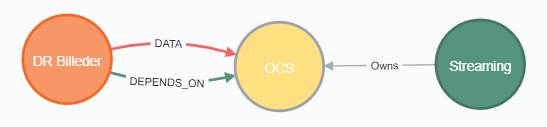
\includegraphics[width=300pt]{OCS.PNG}
\caption{MATCH (x\{name:'OCS'\})- -(y) RETURN x,y}
\end{figure}
\subsubsection{Kort beskrivelse}
API-afløseren til PSDB (MU-online), der leverer video- og radio-data (ikke anvendt i Web \& Apps endnu)	Udstiller program- og seriedata, således at aftagere kan benytte dette til at vise TV/Radio-indhold
\subsubsection{Anbefalet handling}
Ved ændringer i systemer der afhænger af PSDB, så bør det undersøges om det er relevant at anvende OCS i stedet.
\subsubsection{Overslag}
Da OCS ikke ejes af Web og Apps og da ingen systemer afhænger af OCS endnu, så er der ingen indsatser nødvendige på OCS.


\subsection{Garnnøgle}
\begin{figure}[h]
\includegraphics[width=300pt]{Garnnøgle.PNG}
\caption{MATCH (x\{name:'Garnnøgle'\})- -(y) RETURN x,y}
\end{figure}
\subsubsection{Kort beskrivelse}
Tema- og sagskategorisering af artikelindhold, således specielt nyhedsindhold kan inddeles i overordnede kategorier. Bruges også som emnebaseret abonnement-mekanisme i Nyhedsapp
Garnnøgle er ret central i værdikæden for DR.dk, da den benyttes af en lang række systemer og funktioner. Garnnøgle applikationen er behæftet med en del teknisk gæld og unødig kompleksitet i dens implementering.
\subsubsection{Anbefalet handling}
Garnnøgles placering i forhold til referencearkitekturen er ok. Selve implementeringen af garnnøgle bør dog genbesøges og afhængigt af det reelle forretningsbehov skal vi have set på en ny implementering.
\subsubsection{Overslag}
Udvikling af ny garnnøgle: Grov estimat 8 mandeuger.


\subsection{Drupal}
\begin{figure}[h]
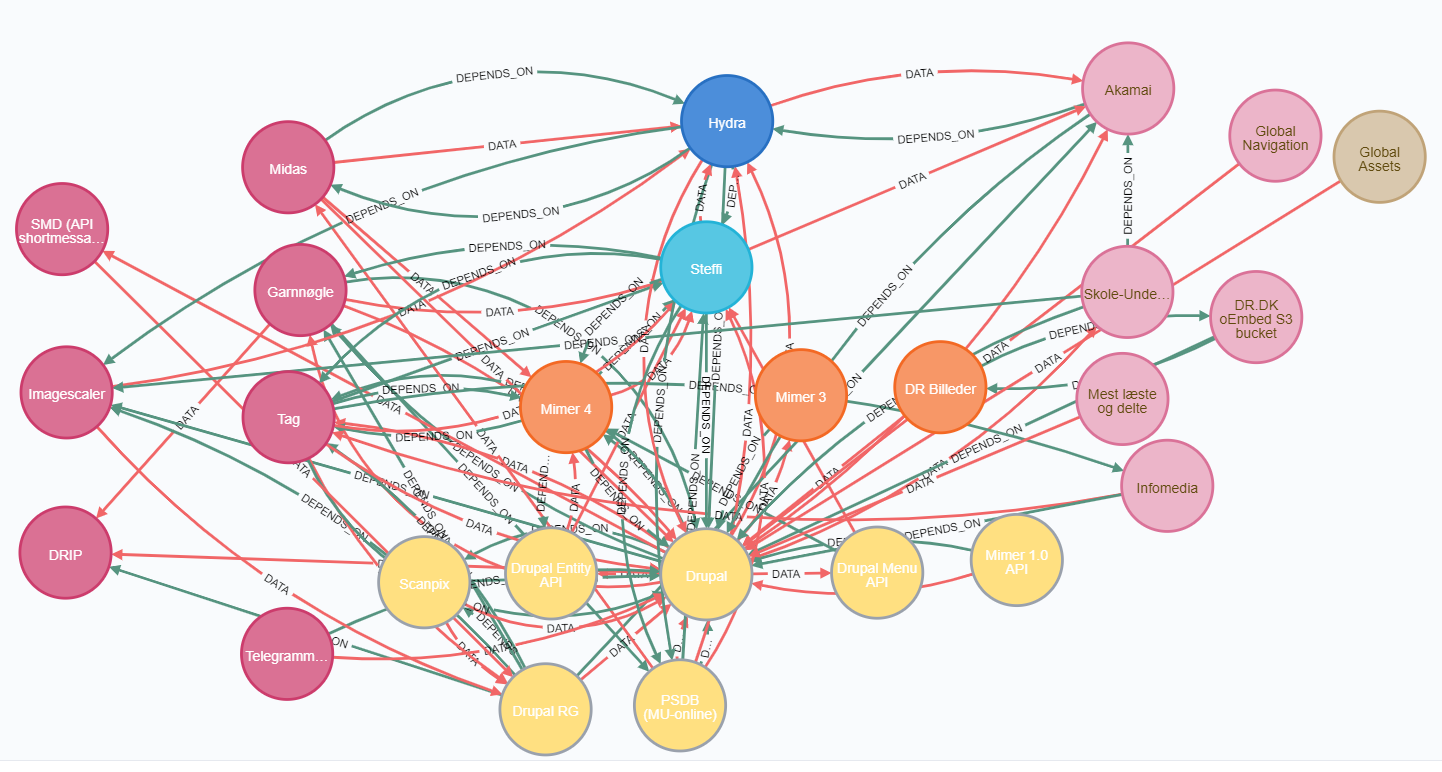
\includegraphics[width=300pt]{Drupal.PNG}
\caption{MATCH (x\{name:'Drupal'\})- -(y) RETURN x,y}
\end{figure}
\subsubsection{Kort beskrivelse}
Det primære CMS til tekstbaseret indhold på DR.dk, samt redaktionel grænseflade til indholdsproduktion og slutteligt mulighed for at grafisk opbygge sektionsforsider og sites.
\subsubsection{Anbefalet handling}
I henhold til referencearkitekturen burde Drupal kun være forbundet med Content Services og Platform Services. Da Drupal er det centrale CMS system er antallet af forbindelser ikke den store overraskelse, det peger dog entydigt på at DR stadig er meget hængt op på Drupal og dermed vil en eventuel udskiftning eller opdatering af Drupal være en stor udgift.
Vi bør helt klart se på at nedbringe antallet af direkte afhængigheder til og fra Drupal. 
Dette kan enten ske ved at lade Platform Services snakke med Content Services (f.eks. at lade garnnøgle afhænge af Mimer i stedet for Drupal), affolke og lukke de gamle udgaver af Mimer eller sikre at kun services med en god grund kan kommunikere med Drupal.

Drupal er lige nu vores styrende CMS system, det vil sige at Drupal har kontrollen med alle URL hos DR.dk, hvilket også er grunden til den direkte forbindelse fra Hydra ned til Drupal. Det vil være meget fornuftigt at kikke på at få etableret et fornuftigt URN / URL system, således at en URL / URN i sig selv er beskrivende nok til at kunne udpege det styrende indholdssystem. Det vil muliggøre sideløbende CMS systemer med hvert deres fokus og gøre det lettere at opdatere / udskifte Drupal på sigt.
 
Vi skal også have kikket på roadmap for opdatering af Drupal 7 til enten Drupal 8 eller et andet CMS system. Drupal 7 (vores nuværende installation) har end of life i november 2021.
\subsubsection{Overslag}
Migrering fra Drupal 7 til andet CMS system vil være en betydelig opgave, især med det niveau af afhængigheder og egenudvikling der er foretaget på Drupal platformen. 
Selve analysen af tidsforbrug for skiftet er uden for scope af denne rapport. Hvis vi går ud fra at det giver mening at skifte direkte fra Drupal 7 til 9 kan et groft overslag 300+ timer. Vi vil få brug for ekstern hjælp.

URN / URL 


\subsection{Mimer 1.0 API}
\begin{figure}[h]
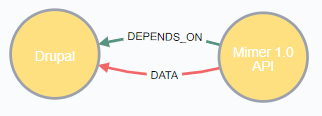
\includegraphics[width=200pt]{MimerAPI.PNG}
\caption{MATCH (x\{name:'Mimer 1.0 API'\})- -(y) RETURN x,y}
\end{figure}
\subsubsection{Kort beskrivelse}
Mimer 1.0 API er nogle REST services i Drupal, som giver Mimer 1.1 adgang til at oprette nyt indhold.
\subsubsection{Anbefalet handling}
Mimer 1.0 API er allerede under afvikling. Denne afvikling bør fortsættes og systemet lukkes.
\subsubsection{Overslag}
N/A

\subsection{Drupal RG}
\begin{figure}[h]
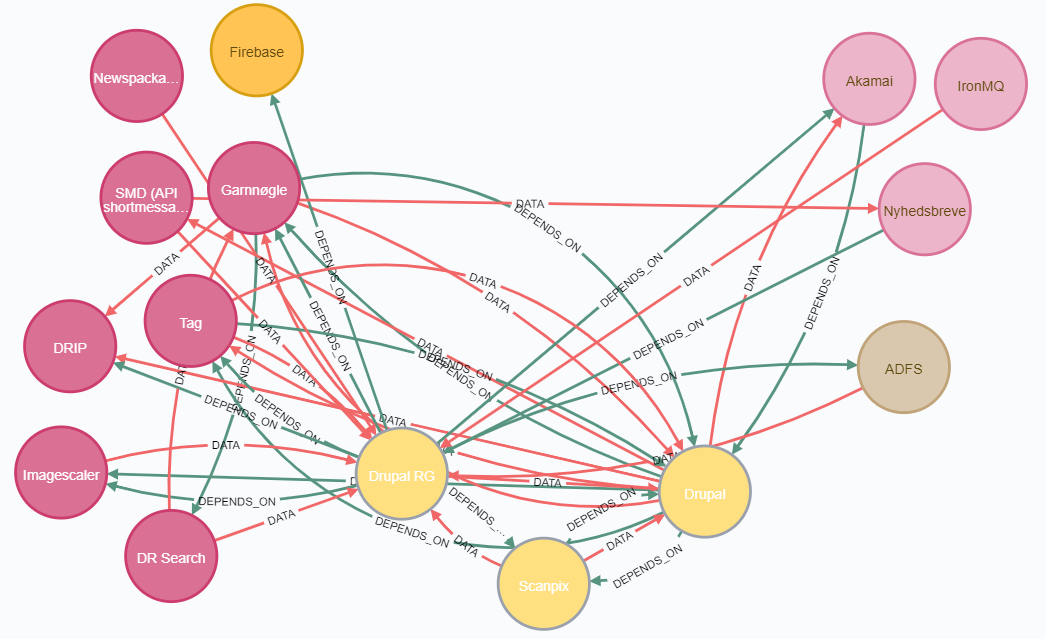
\includegraphics[width=300pt]{DrupalRG.PNG}
\caption{MATCH (x\{name:'Drupal RG'\})- -(y) RETURN x,y}
\end{figure}
\subsubsection{Kort beskrivelse}
Nyeste version af redaktør grænsefladen, lanceret Q1-2018. Redaktør grænsefladen (RG) er journalisternes værktøj til artikelproduktion. Den findes i to udgaver, hhv. RG1 og RG2.	

Webbaseret grænseflade til at oprette, redigere og distribuere tekstbaseret indhold, primært artikler. Tilbyder også integration med tema, kategoriserings, og push-funktioner.
\subsubsection{Anbefalet handling}
%TODO
\subsubsection{Overslag}


\subsection{Drupal Entity API}
\begin{figure}[h]
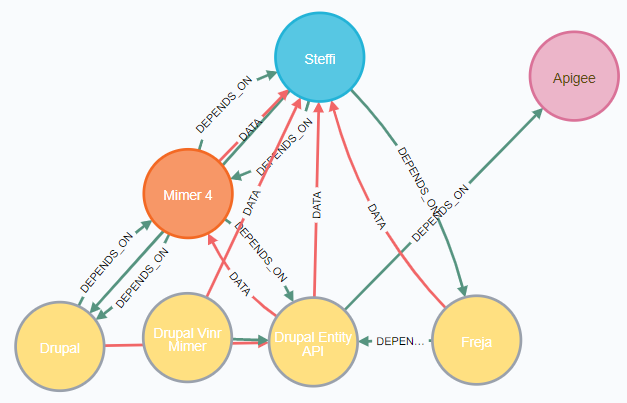
\includegraphics[width=300pt]{DrupalEntityAPI.PNG}
\caption{MATCH (x\{name:'Drupal Entity API'\})- -(y) RETURN x,y}
\end{figure}
\subsubsection{Kort beskrivelse}
Udstiller væsentlige dele af Drupals datamodel for indholdstyper i et simpelt API
\subsubsection{Anbefalet handling}
%TODO
\subsubsection{Overslag}



\subsection{Drupal Menu API}
\begin{figure}[h]
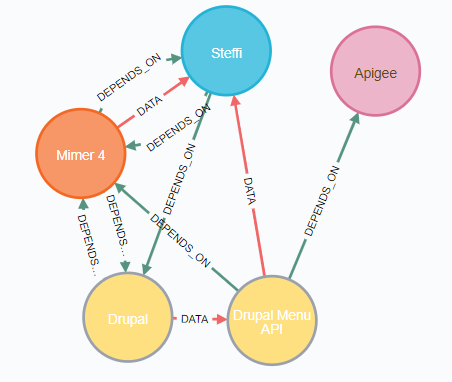
\includegraphics[width=300pt]{DrupalMenuAPI.PNG}
\caption{MATCH (x\{name:'Drupal Menu API'\})- -(y) RETURN x,y}
\end{figure}
\subsubsection{Kort beskrivelse}
Udstiller Drupals menu og sitestruktur til aftagere, der ønsker at præsentere indhold i en hierarkisk visning.
\subsubsection{Anbefalet handling}
%TODO
\subsubsection{Overslag}


\subsection{Ensighten}
\begin{figure}[h]
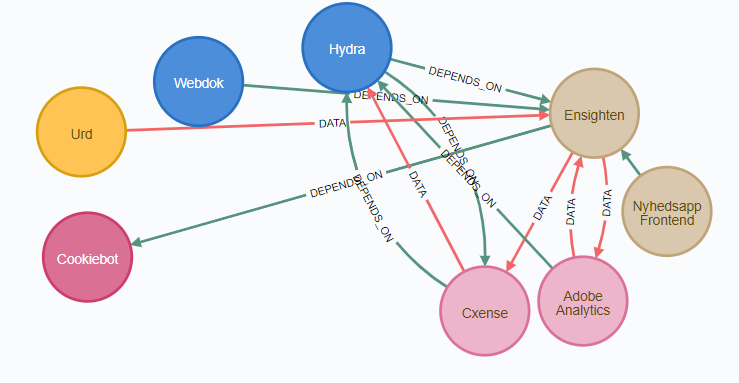
\includegraphics[width=250pt]{Ensighten.PNG}
\caption{MATCH (x\{name:'Ensighten'\})- -(y) RETURN x,y}
\end{figure}
\subsubsection{Kort beskrivelse}
Indskyder JavaScript på dr.dk sider, f.eks. til analytics, bannere, mv. Sørger derudover også for at hente og behandle metadata til analytics og anbefalingssystemer.
\subsubsection{Anbefalet handling}
\subsubsection{Overslag}


\subsection{Ad Server}
\subsubsection{Kort beskrivelse}
"Smart Ad Server" er en hosted løsning, hvor bannerhåndtering og booking/kampagner bliver håndteret. Integreres med DR applikationer der skal vise bannere til slutbrugere.
\subsubsection{Anbefalet handling}
SaaS. Der er ingen udviklingsmuligheder her, kun eventuelt at fjerne afhængigheden heraf hvis nødvendigt.
\subsubsection{Overslag}


\subsection{Midas}
\begin{figure}[h]
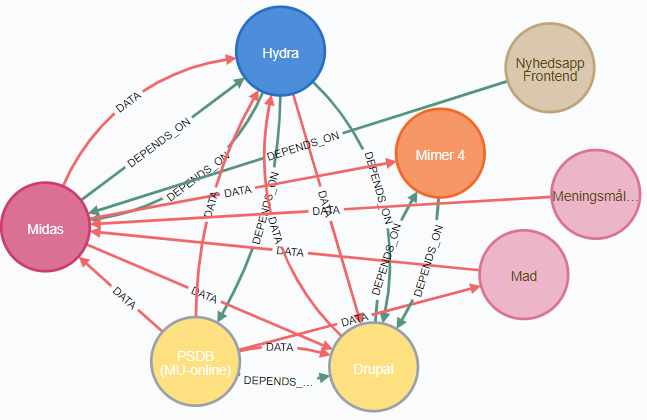
\includegraphics[width=200pt]{Midas.PNG}
\caption{MATCH (x\{name:'Midas'\})- -(y) RETURN x,y}
\end{figure}
\subsubsection{Kort beskrivelse}
Oembed-service, der omsætter oEmbed-referencer til markup, til brug i frontend.
\subsubsection{Anbefalet handling}
\subsubsection{Overslag}


\subsection{PSDB (MU-online)}
\begin{figure}[h]
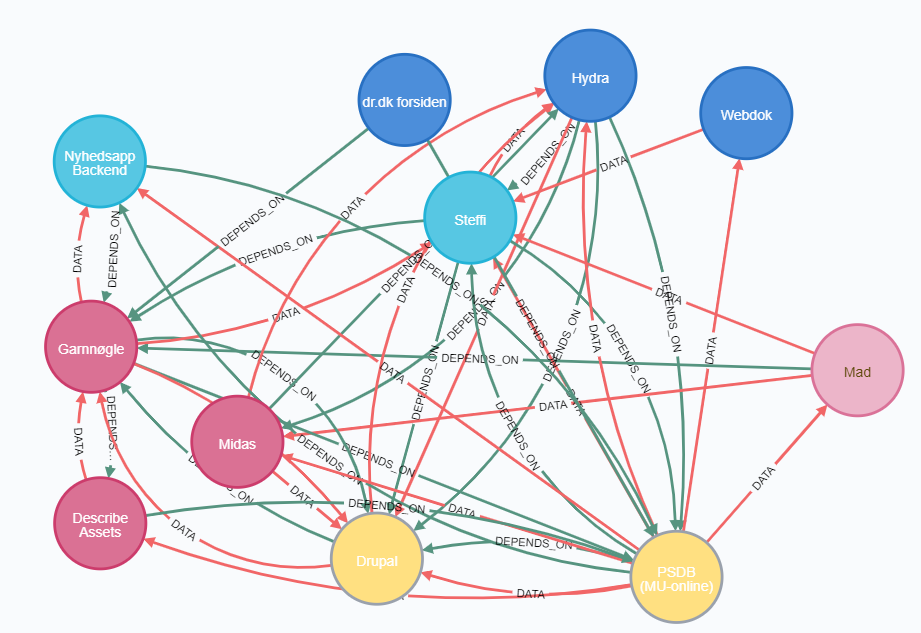
\includegraphics[width=300pt]{PSDB.PNG}
\caption{MATCH (x\{name:'PSDB (MU-online)'\})- -(y) RETURN x,y}
\end{figure}
\subsubsection{Kort beskrivelse}
Program og seriedatabase til TV-baseret indhold
\subsubsection{Anbefalet handling}
Ejerskabet af dette system ligger uden for Web og Apps.
\subsubsection{Overslag}


\subsection{Scanpix}
\begin{figure}[h]
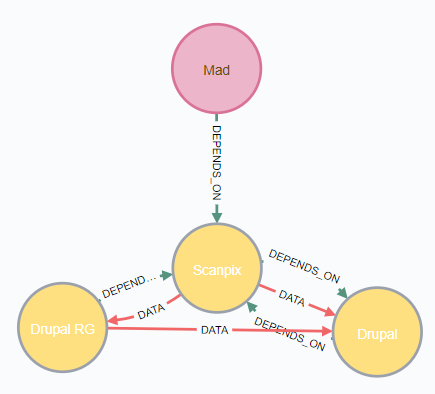
\includegraphics[width=160pt]{Scanpix.PNG}
\caption{MATCH (x\{name:'Scanpix'\})- -(y) RETURN x,y}
\end{figure}
\subsubsection{Kort beskrivelse}
Billededatabase. Ekstern service, der tilbyder redaktører at søge efter billed- og videoindhold som kan importeres og anvendes i DR's systemer.
\subsubsection{Anbefalet handling}
SaaS. Der er ingen udviklingsmuligheder her, kun eventuelt at fjerne afhængigheden heraf hvis nødvendigt.
\subsubsection{Overslag}


\subsection{Cxense}
\begin{figure}[h]
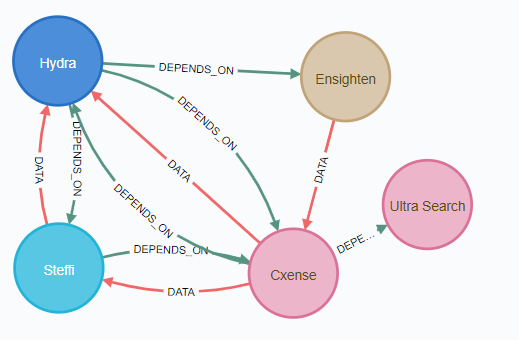
\includegraphics[width=200pt]{Cxense.PNG}
\caption{MATCH (x\{name:'Cxense'\})- -(y) RETURN x,y}
\end{figure}
\subsubsection{Kort beskrivelse}
Analysesystem til personalisering
\subsubsection{Anbefalet handling}
SaaS. Der er ingen udviklingsmuligheder her, kun eventuelt at fjerne afhængigheden heraf hvis nødvendigt.
\subsubsection{Overslag}


\subsection{Adobe Analytics}
\begin{figure}[h]
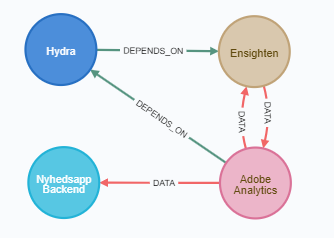
\includegraphics[width=200pt]{AdobeAnalytics.PNG}
\caption{MATCH (x\{name:'Adobe Analytics'\})- -(y) RETURN x,y}
\end{figure}
\subsubsection{Kort beskrivelse}
Analysesystem til personalisering
\subsubsection{Anbefalet handling}
SaaS. Der er ingen udviklingsmuligheder her, kun eventuelt at fjerne afhængigheden heraf hvis nødvendigt.
\subsubsection{Overslag}


\subsection{Pressebilleder}
\subsubsection{Kort beskrivelse}
Pressesite på dr.dk Udsendelse af nyhedsbreve, integration til Mosaic-billeddatabase. Sandsynligvis eksternt produkt.
\subsubsection{Anbefalet handling}
N/A
\subsubsection{Overslag}
N/A

\subsection{WebCMS}
\begin{figure}[h]
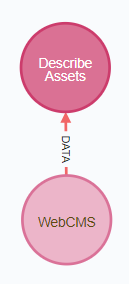
\includegraphics[height=120pt]{WebCMS.PNG}
\caption{MATCH (x\{name:'WebCMS'\})- -(y) RETURN x,y}
\end{figure}
\subsubsection{Kort beskrivelse}
Content Management System håndtering af sider på dr.dk. Udfaset og afløst af Drupal.
\subsubsection{Anbefalet handling}
N/A
\subsubsection{Overslag}
N/A

\subsection{DR Search}
\begin{figure}[h]
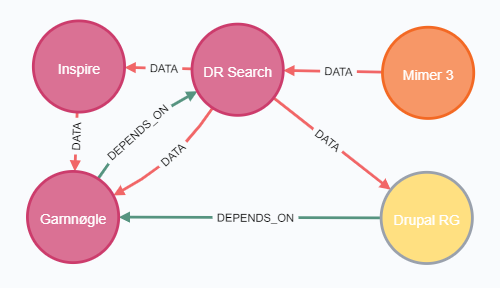
\includegraphics[width=200pt]{DRSearch.PNG}
\caption{MATCH (x\{name:'DR Search'\})- -(y) RETURN x,y}
\end{figure}
\subsubsection{Kort beskrivelse}
Søgemaskine tekst, video og radioindhold på DR.dk	

Tilbyder søgefunktionalitet med ekstrem domæneforståelse for DR's forskellige indholdstyper, distributionsregler og indholdssystemer. Kan indlejres i RG-systemer og tilbyde specialiseret søgefunktionalitet til både publiceret og ikke-publiceret indhold. Kan tilbyde slutbrugere at søge agnostisk og præsenterer søgeresultater ud fra den type indhold der er tale om, eks afspilningsoplysninger til TV-indhold. Indekserer de forskellige indholdssystemer for nyt eller opdateret indhold, og indekserer også indhold via webvisning på DR.dk
\subsubsection{Anbefalet handling}
DR Search er for tiden uden ejerskab og uden ansvarlige udviklere. Enten skal systemet adopteres af at team eller også så skal vi have afviklet systemet. Der er ikke umiddelbart et system der kan tage over som erstatning for DR Search endnu. 

%TODO 
* Skal vi erstatte?
* Skal vi beholde?
* Skal det helt skrottes?
* Kan vi benytte Drupals search til artiker, og evt streamingtjenestens søgefunktionalitet til TV / Radio?
\subsubsection{Overslag}


\subsection{Nyhedsbreve}
\begin{figure}[h]
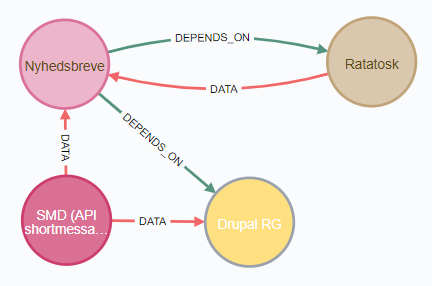
\includegraphics[width=200pt]{Nyhedsbreve.PNG}
\caption{MATCH (x\{name:'Nyhedsbreve'\})- -(y) RETURN x,y}
\end{figure}
\subsubsection{Kort beskrivelse}
Udsendelse af nyhedsbreve. Benytter Peytz' service	

Tilbyder nyhedsbreve som en distributionskanal til DR's indholdsysstemer, således at indhold kan skubbes ud til brugeren samtidig med at det publiceres på DR.dk
\subsubsection{Anbefalet handling}
SaaS men uden ejerskab. 
Det skal vurderes om denne løsning er passende for vores fremtidige arkitektur. Det er dog ikke højeste prioritet.
\subsubsection{Overslag}


\subsection{DR Billeder}
\begin{figure}[h]
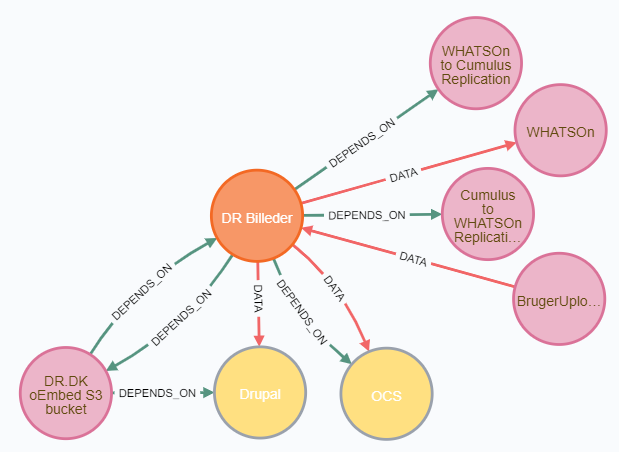
\includegraphics[width=200pt]{DRBilleder.PNG}
\caption{MATCH (x\{name:'DR Billeder'\})- -(y) RETURN x,y}
\end{figure}
\subsubsection{Kort beskrivelse}
Billedhåndteringssystem til DR's indholdsproducenter, anvender standardsystemet Cumulus fra Canto. Der anvendes en underleverandør, Attention, til at konfigurere systemet. Består af følgende delkomponenter: Database, applikationsserver, web UI, tyk klient.
\subsubsection{Anbefalet handling}
Ingen handling nødvendig. Systemet håndteres uden for Web og Apps
\subsubsection{Overslag}


\subsection{DR.DK oEmbed S3 bucket}
\begin{figure}[h]
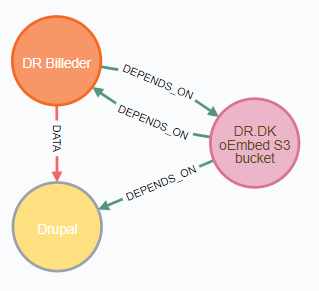
\includegraphics[width=120pt]{S3Bucket.PNG}
\caption{MATCH (x\{name:'DR.DK oEmbed S3 bucket'\})- -(y) RETURN x,y}
\end{figure}
\subsubsection{Kort beskrivelse}
En AWS S3 bucket der anvendes til online versioner af billeder som indlejres med oEmbed
\subsubsection{Anbefalet handling}
Ingen handling nødvendig. Systemet håndteres uden for Web og Apps
\subsubsection{Overslag}


\subsection{Mimer 3}
\begin{figure}[h]
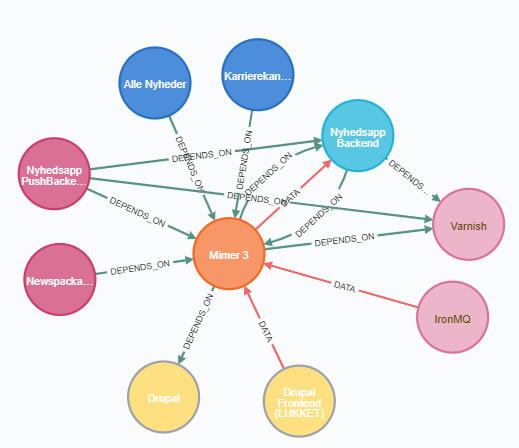
\includegraphics[width=300pt]{Mimer3.PNG}
\caption{MATCH (x\{name:'Mimer 3'\})- -(y) RETURN x,y}
\end{figure}
\subsubsection{Kort beskrivelse}
API til Drupals artikelindhold.

Udstiller Drupals primære indholdstyper til brug og visning i andre systemer.
\subsubsection{Anbefalet handling}
Mimer 3 er under afvikling. Det viste billede af afhængigheder er stadig ved at skrumpe. Mimer 3 bør afvikles helt og fjernes, så vi slipper for at have parallelle implementeringer der løser de samme opgaver.
\subsubsection{Overslag}
Der mangler stadig mange afhængigheder der skal migreres over på Mimer 4. Disse er dog i pipeline.


\subsection{Mimer 4}
\begin{figure}[h]
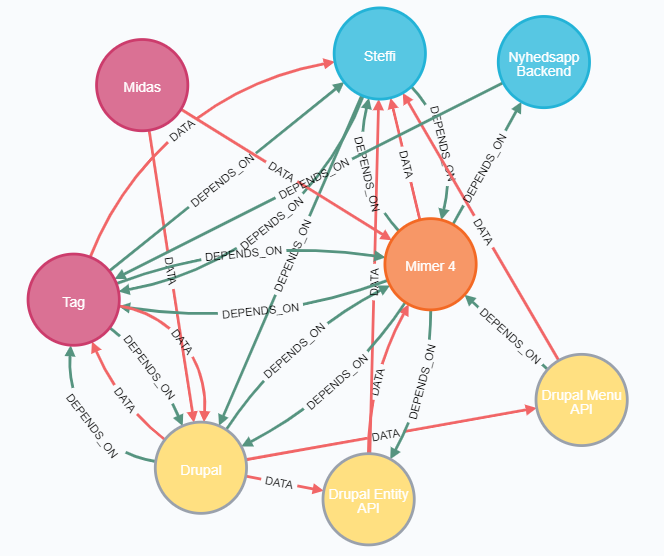
\includegraphics[width=200pt]{Mimer4.PNG}
\caption{MATCH (x\{name:'Mimer 4'\})- -(y) RETURN x,y}
\end{figure}
\subsubsection{Kort beskrivelse}
API til Drupals artikelindhold.

Udstiller Drupals primære indholdstyper til brug og visning i andre systemer.
\subsubsection{Anbefalet handling}
\subsubsection{Overslag}


\subsection{Tag}
\begin{figure}[h]
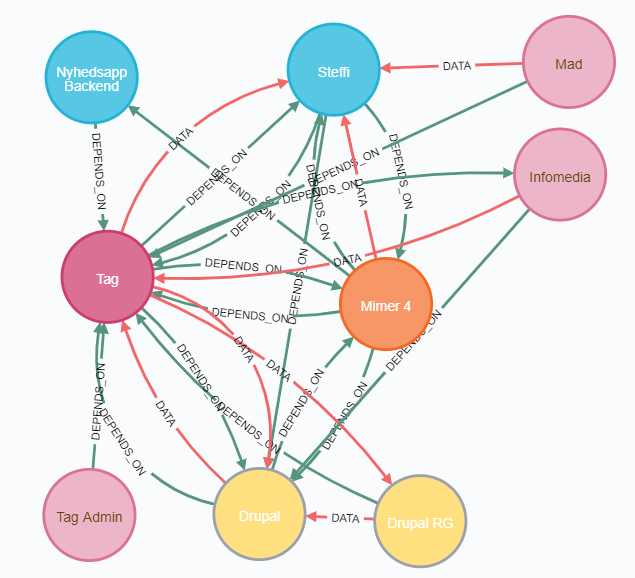
\includegraphics[width=200pt]{Tag.PNG}
\caption{MATCH (x\{name:'Tag'\})- -(y) RETURN x,y}
\end{figure}
\subsubsection{Kort beskrivelse}
Tagsystem til opmærkning af DR's web-indhold.
\subsubsection{Anbefalet handling}
Tag manager systemet bliver slet ikke brugt i det omfang det burde. Sidste opdatering er fra marts 2018. Vi bør sammen med opdateringen af garnnøgle se på om vi kan enten bygge Tag systemet sammen med Garnnøgles erstatning eller helt udskifte Tag systemet til noget der stemmer mere overens med de behov vi har.
\subsubsection{Overslag}


\subsection{Urd}
\begin{figure}[h]
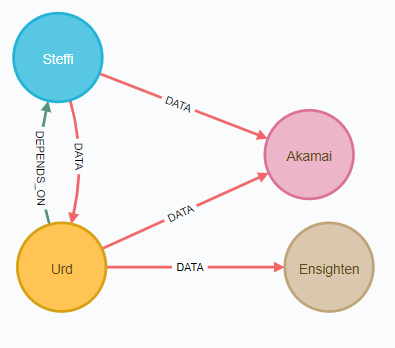
\includegraphics[width=160pt]{Urd.PNG}
\caption{MATCH (x\{name:'Urd'\})- -(y) RETURN x,y}
\end{figure}
\subsubsection{Kort beskrivelse}
Metadataservice, der leverer metadata til brug i TMS
\subsubsection{Anbefalet handling}
\subsubsection{Overslag}


\subsection{Infomedia}
\begin{figure}[h]
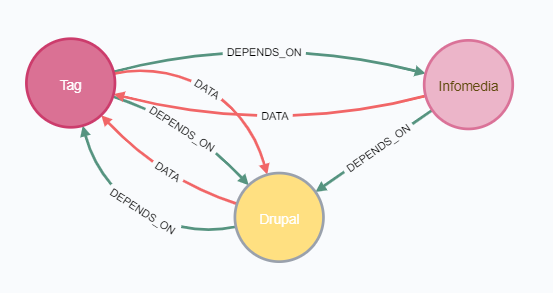
\includegraphics[width=300pt]{Infomedia.PNG}
\caption{MATCH (x\{name:'Infomedia'\})- -(y) RETURN x,y}
\end{figure}
\subsubsection{Kort beskrivelse}
Taksonomidatabase og tekstanalysesystem til tags.

Tilbyder en komplet, vedligeholdt taksonomi samt tekstanalysefunktionalitet, der kan analysere en given tekst og indikere tags fra taksonomien som er relevante.

\subsubsection{Anbefalet handling}
Infomedia bruges idag til tag systemet. Tag systemet og Garnnøgle står formentligt over for en større omskrivning. Om Infomedia skal benyttes til tekstanalyse og forslag til Tagging af artikler skal vi have set nærmere på.
\subsubsection{Overslag}


\subsection{Auth0}
\begin{figure}[h]
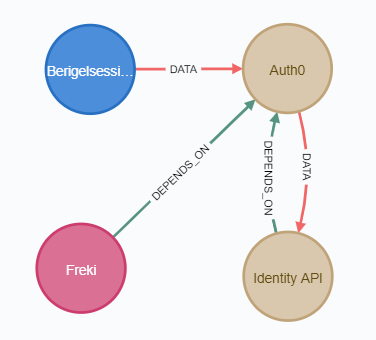
\includegraphics[width=130pt]{Auth0.PNG}
\caption{MATCH (x\{name:'Auth0'\})- -(y) RETURN x,y}
\end{figure}
\subsubsection{Kort beskrivelse}
Oauth autentifikations platform. SaaS.
\subsubsection{Anbefalet handling}
Auth0 er en fin platform til autentificering af brugere. Det er en betalt service, der passer godt ind i vores eksisterende programstak. 
\subsubsection{Overslag}
N/A


\subsection{Identity API}
\begin{figure}[h]

\includegraphics[width=300pt]{CHANGE.PNG}
\caption{MATCH (x\{name:'CHANGE'\})- -(y) RETURN x,y}
\end{figure}
\subsubsection{Kort beskrivelse}
Backend til DR's login-løsning.
\subsubsection{Anbefalet handling}
Ingen nødvendig
\subsubsection{Overslag}
N/A

\subsection{Telegrammaskine}
\begin{figure}[h]
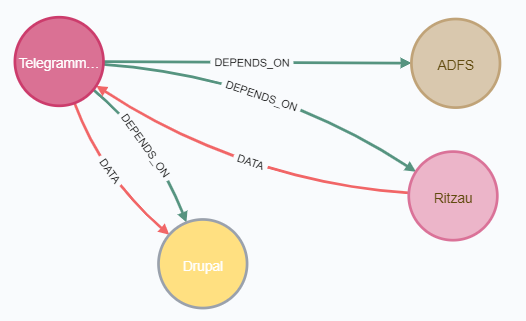
\includegraphics[width=300pt]{Telegrammaskine.PNG}
\caption{MATCH (x\{name:'Telegrammaskine'\})- -(y) RETURN x,y}
\end{figure}
\subsubsection{Kort beskrivelse}
Integration til Ritzau-indhold, med mulighed for at redigere og udgive telegrammer som Drupal-artikler.	

DR modtager løbende nyhedsunderretninger fra Ritzau i form af telegrammer; Telegrammaskinen tilbyder redaktører en meget hurtig måde at overskue seneste telegrammer samt at publicere disse direkte på DR.dk
\subsubsection{Anbefalet handling}
Ingen ændringer nødvendigt.
\subsubsection{Overslag}
N/A

\subsection{Dr. Edition}
\begin{figure}[h]
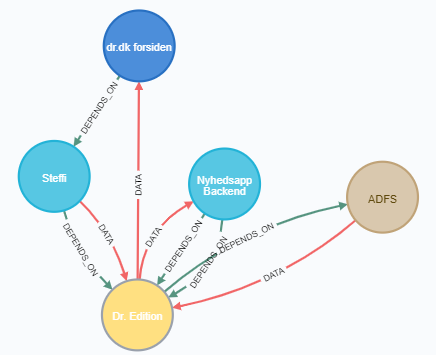
\includegraphics[width=300pt]{DrEdition.PNG}
\caption{MATCH (x\{name:'Dr. Edition'\})- -(y) RETURN x,y}
\end{figure}
\subsubsection{Kort beskrivelse}
Forsideværktøj til forsiden af DR.dk, hvor redaktører udarbejder forsider, inkluderer også API. Benytter Aptomas Dr. Edition-produkt. (steffi kommer snart til at trække til den nye forside). 

Tilbyder forsideredaktører at opbygge og redigere forsiden af DR.dk ud fra seneste udgivne artikelindhold fra Drupal, samt at versionere og skifte mellem flere forskellige forsideudgaver.
\subsubsection{Anbefalet handling}
\subsubsection{Overslag}


\subsection{dr.dk forsiden}
\begin{figure}[h]
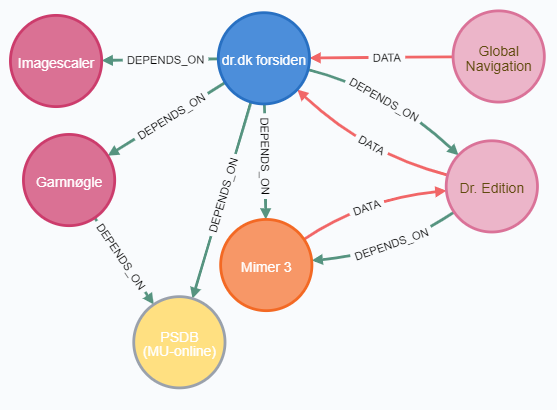
\includegraphics[width=300pt]{DrDkForsiden.PNG}
\caption{MATCH (x\{name:'dr.dk forsiden'\})- -(y) RETURN x,y}
\end{figure}
\subsubsection{Kort beskrivelse}
Azure-driftet ASP.NET MVC applikation til at hente data og vise forsiden af dr.dk

Robust system til visning af de forsider som forsideredaktører udarbejder i Dr. Edition.
\subsubsection{Anbefalet handling}
\subsubsection{Overslag}


\subsection{Alle Nyheder}
\begin{figure}[h]
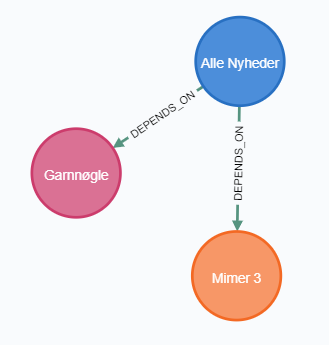
\includegraphics[width=300pt]{AlleNyheder.PNG}
\caption{MATCH (x\{name:'Alle Nyheder'\})- -(y) RETURN x,y}
\end{figure}
\subsubsection{Kort beskrivelse}
Systemet der driver siden allenyheder (alle nyheder): http://www.dr.dk/nyheder/allenyheder/	

Tilbyder overblik over senest publiceret artikelindhold samt en søgning ud fra publiceringstidspunkt
\subsubsection{Anbefalet handling}
\subsubsection{Overslag}


\subsection{Newsapp UI}
\begin{figure}[h]
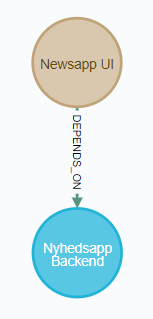
\includegraphics[width=300pt]{NyhedsAppUi.PNG}
\caption{MATCH (x\{name:'Newsapp UI'\})- -(y) RETURN x,y}
\end{figure}
\subsubsection{Kort beskrivelse}
Web-renderingsværktøj til DR Nyheder (app). Web-hostet værktøj til at se mobil app i web-version. Placeret på https://www.dr.dk/tjenester/newsapp-ui/.	

Redaktørvendt visning af hvordan indhold vises i Nyhedsapp, således at redaktører kan lave Nyhedsapp-specifikt preview af indhold.
\subsubsection{Anbefalet handling}
Ingen nødvendig. Applikationen lever eller dør med de 2 nyheds App
\subsubsection{Overslag}
N/A

\subsection{SMD (API shortmessage-dispatcher)}
\begin{figure}[h]
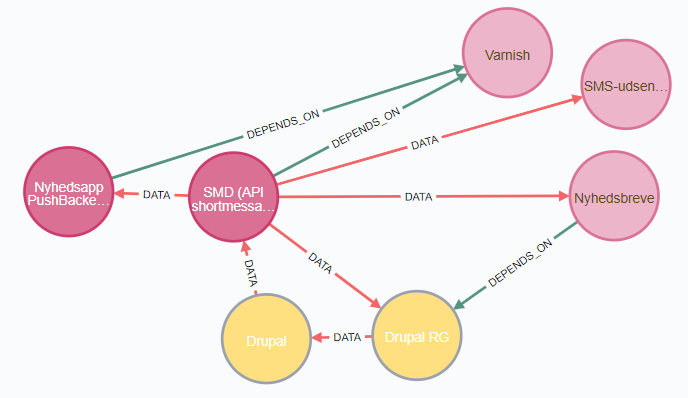
\includegraphics[width=300pt]{SMD.PNG}
\caption{MATCH (x\{name:'SMD (API shortmessage-dispatcher)'\})- -(y) RETURN x,y}
\end{figure}
\subsubsection{Kort beskrivelse}
Push SMS; nyhedsbrev, Nyheds app. fra f.eks. Drupal, facebook.

Tilbyder push af tekstbaseret indhold til en række forskellige platforme og distributionsmekanismer
\subsubsection{Anbefalet handling}
\subsubsection{Overslag}


\subsection{Mest læste og delte}
\begin{figure}[h]
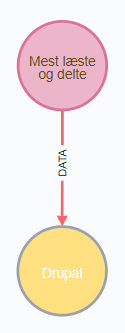
\includegraphics[height=120pt]{MestL.PNG}
\caption{MATCH (x\{name:'Mest læste og delte'\})- -(y) RETURN x,y}
\end{figure}
\subsubsection{Kort beskrivelse}
ESI mest læste og delte mm. på DR.dk og Drupal sider.

Tilbyder en liste af mest besøgt og delt (via social medier) indhold ud fra besøgsstatistik.
\subsubsection{Anbefalet handling}
Applikationen skal lukkes ned, da dens funktionalitet bliver erstattet af Cxense.
\subsubsection{Overslag}


\subsection{Nyhedsapp Backend}
\begin{figure}[h]

\includegraphics[width=300pt]{CHANGE.PNG}
\caption{MATCH (x\{name:'CHANGE'\})- -(y) RETURN x,y}
\end{figure}
\subsubsection{Kort beskrivelse}
\subsubsection{Anbefalet handling}
\subsubsection{Overslag}


\subsection{Tag Admin}
\begin{figure}[h]

\includegraphics[width=300pt]{CHANGE.PNG}
\caption{MATCH (x\{name:'CHANGE'\})- -(y) RETURN x,y}
\end{figure}
\subsubsection{Kort beskrivelse}
\subsubsection{Anbefalet handling}
\subsubsection{Overslag}


\subsection{Ritzau}
\begin{figure}[h]

\includegraphics[width=300pt]{CHANGE.PNG}
\caption{MATCH (x\{name:'CHANGE'\})- -(y) RETURN x,y}
\end{figure}
\subsubsection{Kort beskrivelse}
\subsubsection{Anbefalet handling}
\subsubsection{Overslag}


\subsection{Ratatosk}
\begin{figure}[h]

\includegraphics[width=300pt]{CHANGE.PNG}
\caption{MATCH (x\{name:'CHANGE'\})- -(y) RETURN x,y}
\end{figure}
\subsubsection{Kort beskrivelse}
\subsubsection{Anbefalet handling}
\subsubsection{Overslag}


\subsection{Drupal Vinr Mimer}
\begin{figure}[h]

\includegraphics[width=300pt]{CHANGE.PNG}
\caption{MATCH (x\{name:'CHANGE'\})- -(y) RETURN x,y}
\end{figure}
\subsubsection{Kort beskrivelse}
\subsubsection{Anbefalet handling}
\subsubsection{Overslag}


\subsection{DRIP}
\begin{figure}[h]
\includegraphics[width=300pt]{CHANGE.PNG}
\caption{MATCH (x\{name:'CHANGE'\})- -(y) RETURN x,y}
\end{figure}
\subsubsection{Kort beskrivelse}
\subsubsection{Anbefalet handling}
\subsubsection{Overslag}


\subsection{Global Navigation}
\begin{figure}[h]
\includegraphics[width=300pt]{CHANGE.PNG}
\caption{MATCH (x\{name:'CHANGE'\})- -(y) RETURN x,y}
\end{figure}
\subsubsection{Kort beskrivelse}
\subsubsection{Anbefalet handling}
\subsubsection{Overslag}


\subsection{BrugerUpload}
\begin{figure}[h]
\includegraphics[width=300pt]{CHANGE.PNG}
\caption{MATCH (x\{name:'CHANGE'\})- -(y) RETURN x,y}
\end{figure}
\subsubsection{Kort beskrivelse}
\subsubsection{Anbefalet handling}
\subsubsection{Overslag}


\subsection{Imagescaler}
\begin{figure}[h]
\includegraphics[width=300pt]{CHANGE.PNG}
\caption{MATCH (x\{name:'CHANGE'\})- -(y) RETURN x,y}
\end{figure}
\subsubsection{Kort beskrivelse}
\subsubsection{Anbefalet handling}
\subsubsection{Overslag}


\subsection{ADFS}
\begin{figure}[h]
\includegraphics[width=300pt]{CHANGE.PNG}
\caption{MATCH (x\{name:'CHANGE'\})- -(y) RETURN x,y}
\end{figure}
\subsubsection{Kort beskrivelse}
\subsubsection{Anbefalet handling}
\subsubsection{Overslag}


\subsection{Global Assets}
\begin{figure}[h]
\includegraphics[width=300pt]{CHANGE.PNG}
\caption{MATCH (x\{name:'CHANGE'\})- -(y) RETURN x,y}
\end{figure}
\subsubsection{Kort beskrivelse}
\subsubsection{Anbefalet handling}
\subsubsection{Overslag}


\subsection{Global}
\begin{figure}[h]
\includegraphics[width=300pt]{CHANGE.PNG}
\caption{MATCH (x\{name:'CHANGE'\})- -(y) RETURN x,y}
\end{figure}
\subsubsection{Kort beskrivelse}
\subsubsection{Anbefalet handling}
\subsubsection{Overslag}


\subsection{Webstat}
\begin{figure}[h]
\includegraphics[width=300pt]{CHANGE.PNG}
\caption{MATCH (x\{name:'CHANGE'\})- -(y) RETURN x,y}
\end{figure}
\subsubsection{Kort beskrivelse}
\subsubsection{Anbefalet handling}
\subsubsection{Overslag}


\subsection{Describe Assets}
\begin{figure}[h]
\includegraphics[width=300pt]{CHANGE.PNG}
\caption{MATCH (x\{name:'CHANGE'\})- -(y) RETURN x,y}
\end{figure}
\subsubsection{Kort beskrivelse}
\subsubsection{Anbefalet handling}
\subsubsection{Overslag}


\subsection{URN Router}
\begin{figure}[h]
\includegraphics[width=300pt]{CHANGE.PNG}
\caption{MATCH (x\{name:'CHANGE'\})- -(y) RETURN x,y}
\end{figure}
\subsubsection{Kort beskrivelse}
\subsubsection{Anbefalet handling}
\subsubsection{Overslag}


\subsection{Freja}
\begin{figure}[h]
\includegraphics[width=300pt]{CHANGE.PNG}
\caption{MATCH (x\{name:'CHANGE'\})- -(y) RETURN x,y}
\end{figure}
\subsubsection{Kort beskrivelse}
\subsubsection{Anbefalet handling}
\subsubsection{Overslag}


\subsection{Karrierekanonen}
\begin{figure}[h]
\includegraphics[width=300pt]{CHANGE.PNG}
\caption{MATCH (x\{name:'CHANGE'\})- -(y) RETURN x,y}
\end{figure}
\subsubsection{Kort beskrivelse}
\subsubsection{Anbefalet handling}
\subsubsection{Overslag}


\subsection{Apigee}
\begin{figure}[h]
\includegraphics[width=300pt]{CHANGE.PNG}
\caption{MATCH (x\{name:'CHANGE'\})- -(y) RETURN x,y}
\end{figure}
\subsubsection{Kort beskrivelse}
\subsubsection{Anbefalet handling}
\subsubsection{Overslag}


\subsection{Varnish}
\begin{figure}[h]
\includegraphics[width=300pt]{CHANGE.PNG}
\caption{MATCH (x\{name:'CHANGE'\})- -(y) RETURN x,y}
\end{figure}
\subsubsection{Kort beskrivelse}
\subsubsection{Anbefalet handling}
\subsubsection{Overslag}


\subsection{Newspackage service}
\begin{figure}[h]
\includegraphics[width=300pt]{CHANGE.PNG}
\caption{MATCH (x\{name:'CHANGE'\})- -(y) RETURN x,y}
\end{figure}
\subsubsection{Kort beskrivelse}
\subsubsection{Anbefalet handling}
\subsubsection{Overslag}


\subsection{Freki}
\begin{figure}[h]
\includegraphics[width=300pt]{CHANGE.PNG}
\caption{MATCH (x\{name:'CHANGE'\})- -(y) RETURN x,y}
\end{figure}
\subsubsection{Kort beskrivelse}
\subsubsection{Anbefalet handling}
\subsubsection{Overslag}


\subsection{Berigelsessider}
\begin{figure}[h]
\includegraphics[width=300pt]{CHANGE.PNG}
\caption{MATCH (x\{name:'CHANGE'\})- -(y) RETURN x,y}
\end{figure}
\subsubsection{Kort beskrivelse}
\subsubsection{Anbefalet handling}
\subsubsection{Overslag}


\subsection{IronMQ}
\begin{figure}[h]
\includegraphics[width=300pt]{CHANGE.PNG}
\caption{MATCH (x\{name:'CHANGE'\})- -(y) RETURN x,y}
\end{figure}
\subsubsection{Kort beskrivelse}
\subsubsection{Anbefalet handling}
\subsubsection{Overslag}


\section{Anbefaling}

% Der mangler nok lidt fyld her

\end{document}
